\documentclass{article}

\usepackage{geometry}
\usepackage{graphicx}
\graphicspath{ {./images/} }


\renewcommand{\bf}{\textbf}
\renewcommand{\it}{\textit}

\begin{document}

\begin{center}
{\Large \sc Levels of Abstraction in Machine Learning}
\\[2em]
{\large Henry Blanchette}
\end{center}

% \vspace{2em}
% \begin{abstract}
% % TODO
% \end{abstract}

\vspace{2em}

\section{Introduction}

The techniques of machine learning (ML) in the broader field of artificial intellgence (AI) has undeniably made huge headway recently.
However there still seem to be some significant inadequacies with the state-of-the-art machine \it{intelligence} even for relatively narrow tasks.
For example, modern ML in the form of a convolutional neural network (CNN) has achieved super-human ability in the classic computer game of Breakout, where success is measured by how quickly the algorithm can beat the game.
The CNN achieved this level of skill in Breakout from ``the ground up'', meaning that it was given no special information about the game other that control over input to the game (moving the paddle) and access to the output from the game (looking at the game screen).

A human reader recognize that, in order to gain skill at Breakout, one needs to recognize or learn certain patterns about the physics of the game.
One learns that the ball bounces off the paddle and this is the only way to keep the ball from going out of bounds, and that the ball bounces off of the bricks causing them to disappear and scores a point.
Somewhere along the way, one learns that hollowing out a tunnel through all the brick layers lets the ball bounce around consecutively in the top area scoring lots of points.

But is this how the CNN learned to play? Are there analogous concepts of \it{ball}, \it{paddle}, \it{brick}, and \it{tunnel} represented within the neural network?
One way to probe for answers is to change some feature of the game that requires the player to make use of one of these abstractions in order to readjust their strategy.
And this is where the CNN exposes the fact that the knowledge that it has in the form of intricate weighted connections between nodes in its layers may not likely resemble anything like we'd expect from a human that is considered knowledgable or skilled at breakout.
If the game is modified so that the paddle is slightly higher on the vertical, a human player will have no trouble recognizing how to control this paddle and apply the same skills that they may have learned from the normal version of the game (e.g. tunneling).
But the CNN utterly fails at this task.
When the paddle is moved, it loses all apparently skill at the game.
When it is trained on the new version of the game, starting from its previously-skilled configuration of weights, it basically scrambles its weights randomly before it re-achieves its previous level of skill.
The CNN was unable to salvage any of its knowledge when it needed to account for even such a minor change.

The significance of this observation is that it suggest the CNN likely didn't \it{understand} the game of Breakout in the same way we expect a human to understand the game, even though the CNN was super-human in performance. There are many other examples of this phenomenon, that Melanie brought up during her visit, such as how an image classifier CNN can become highly-proficient at recognizing images of, say, cows, yet when presented with an empty field of grass the CNN still sees cows. Or in some of the more extreme examples, one can engineer a \it{adversarial example} that is carefully designed to take advantage of an image classifier CNN's trained structure to make it recognize whatever the designer wishes in an image while making the image appear relatively unchanged to a human viewers.

\section{Levels of Abstraction}

Recalling the Breakout case, the obvious question to ask of the CNN is ``if the CNN didn't learn even basic abstractions like \it{the paddle}, then what \it{did} the CNN learn that allowed it to play so amazing well?'' While it is possible that CNN learned a few human-recognizable abstractions, the fact that it misses many that humans would find fundamental to undestanding (e.g. the abstraction of \it{the paddle}) suggests that the CNN probably didn't learn many.
In some way the CNN must have found an extremely superficial way to understand Breakout, but still well enough to impress human players who do have a demonstrably deeper understanding.

A simple and likely explanation for the CNN's behavior that accounts for its pattern-obliviousness is that it discovered a sort of ``cheat'' in the form of statistical correlations between certain inputs (pixels and game moves) that were easier to learn that the higher-order abstractions that humans find intuitive and typically expect from a good player (human or otherwise).
The fact that the first significant attempts at designing intelligent systems was a symbolic approach, where human-intuitive patterns were \it{hard-coded} into the system. For example. early chess-player AIs needed hueristics such as ``treat the queen as having a relative value of 9 when evaluating piece trade-offs'' explicity represented in their desicion function).

A human reader should find it obvious that a human player attempting to learn Breakout can skip many of the early steps that were outlined, such as ``the ball bounces off the paddleand this is the only way to keep the ball from going out of bounds.''
A human can look at the Breakout game for less than a second and just know intuitively that the colored disk that is translated across the pixels of the game screen is an individual \it{object} and that it will \it{bounce} off of the boundaries of the screen and the bricks at the top in such a way that the angle of inflection will equal the angle of refraction of the collision.
Humans are expected to have a sort of intuitive physics and concept of object-ness (among other concepts) that a CNN (at least, before training) is not expected to have.
In this way, a continuation of the explanation for the CNN's failure to handle a displaced paddle is that, as an example concept, the pattern of the paddle as a persistent object was never developed withing the CNN's internal representation of Breakout.

Furthermore, it could be possible that such a concept of the paddle is not required for humans to play Breakout well either; the fact that humans apply the concept of \it{object} to the paddle could be completely accidental, negligible, or even inhibitory to the ability of a human to, in principal, excel at Breakout.
As the CNN demonstrates, the ability to play the unmodified version of Breakout at an expert level clearly does not neccessarily require such a conceptualization.
I use the example of the \it{object} concept of the paddle because it seems an intuitively plausible explanation but I have not tested that hypothesis and am not aware of other's having tested it either. My argument relies just on the fact that there is \it{some} concept that humans intuitively use when playing Breakout that they did not typically learn by playing Breakout --- a concept which the CNN ends up not learning and is only manifested in bad play when the game is modified in a way that requires the concept for adaptation.
The question of how humans developed the sorts of intuitions that have been invoked is a very interesting one, and will be addressed later.

So far it has been established that CNNs lack some higher-order intuitions about the tasks on which they are trained. They way that a CNN can still achieve prowess at its designated tasks have been referred to as ``cheats,'' in the form of superficial statistical and correlations between inputs, as opposed to true, deeper understanding.
These ``cheats'' are examples of \bf{first-order patterns}.
A first-order pattern is one that relies exactly on the values of the first-order information about inputs i.e. the first layer of the CNN.
Respectively, \bf{higher-order patterns} are those that rely on the exact values of higher-order inputs (in some heirarchy of abstract) i.e. the deeper layers of the CNN (so, there could be second-order, third-order, etc.\footnote{Though this heirarchy may seem well-defined in how I present it, I intentionally make the distinction just between first-order and higher-order. I suspect that the representation of higher-order patterns within a CNN (or a generic neural network) will have significant iterplay between, say, the 10th and 11th layers. In this way, there is decreasing significance to the distinction between layers the deeper you go. Again, I focus mainly the distinction on that between the first layer and those beyond because this is where the distinction is the most significant (given this \it{decreasing returns on abstraction} model) and also relates most specifically to concrete explanation and experimentation; artificial intelligence researches still consider the human interpretation of the patterns that CNNs do learn to be a massive open problem.}).

The first layer has a unique node for each feature that is fed to the CNN.
For example, if the input is an $(m \times n)$-pixel image then each node of the first layer corresponds the red-green-blue (RGB) value of one of the $mn$ pixels.
Due to the structure of a CNN, most first-order patterns are easier to \it{learn} (train to optimize using the typical training procedures of CNNs) than most higher-order patterns.
This is because the weights of the network are initialized randomly and raw inputs are given to the first layer.

Consider the following toy example of a first-order pattern (which is also used in an experiment layer) just to demonstrate the point.
Suppose there is a CNN with an input layer, $x$ internal fully-connected layers, and an output layer that consists of two nodes (the output nodes).
The first output node indicates the relative probability that the inputted image is solid black, and the second output node indicates the relative probability that it is not solid black.
If $x$ was $0$ i.e. there are no internal layers, then the CNN just needs to independently maximize each of the weights of connections going into the first output node and independelty minimize each of the weights going into the second.
This maximization is very easy for a gradient-descent training procedure (the typical training procedure) because it is exactly monotonic --- there is no interaction between features (pixel values).
However for each layer layer added into the network ($x > 0$),
the same kind of process happens but is just slowed down and buffered by the noise that the added layers introduce.

Observe that it is not, in principal, impossible for the CNN in this example to use the deeper layers to develop abstractions e.g. one node in the 10th layer sums the number of black pixels on the left half of the image and a different node in the 10th layer sums hte number of white pixels on right half of the image.
The key result is just that these sorts of abstractions are improbable, and more efficient weightings that do not develop such abstractions will be trained to first in the training process.
Even in the case that there exist some more efficient higher-order abstractions, if training reaches a local maximum using low-order abstraction it is not always likely and often unlikely that the training will ever deviate towards the former.

% TODO: include this in conclusions or instead here? idk, I think conclusions will be more about the actual experiment rather than my preliminary theory.

This line of thinking points to a simple explanation for the \it{frame problem}.
The frame problem is that of developing AI that is just as adept as current narrow AI but also able to apply its learned skill generally (at least, as generally as humans seem to do).
The seeming paradox that superhuman Breakout-playing CNN can't even deal with a slight change of paddle height is resolved by the (previous) explanation that the human conception of the paddle is not likely very important for becoming Breakout-adept, and that there's no reasons to expect the CNN to learn such a thing given this (in addition to the fact that it never trained with this Breakout variant).
In fact, I would go further to say that the fact that CNNs can so quickly become so good at Breakout without some concepts that humans consider fundamental and intuitive is evidence that such concepts are inhibitory for playing the game best.
Considering beyond just breakout, this argument applies broadly to any task for which CNNs succeed on test on training scenarios but fail on generalized scenarios.
The presence of many general (often higher-order) patterns that humans intuitively pick up have little reason, on their own, to predict the (optimized to be lower-order) patterns that CNNs optimize.

This explanation, however, does not provide a clear path forward for how to solve the frame problem.
The next section describes an experiment that aims to explore one possible solution that keeps the previous explanation of the frame problem in mind.

\section{Incentivizing Abstraction}

As is clear in the Breakout case, on obvious way to force an AI to learn some higher-order pattern is to introduce that pattern explicitly as variance in the training.
So in the Breakout case, a way to make the AI learn to deal with paddles at different heights would be to modify the game it trained on to have the paddle at a random height each game. This slows down the training process a bit, but when all is said and done the pattern will have been learned.
The problem with this approach to teaching higher-order patterns to AIs is that it falls into the same traps as symbolic approaches.
This is because the higher-order pattern must be \it{explicity} introduced into the training data.
In this way, the same symbolic approach from early AI is applied to the training data rather than the AI algorithm itself.
So the engineer training the AI, in the symbolic way, would need to explicity come up with all the higher-order patterns they want to teach the AI and embed them in the training data themselves.
The ideal solution to the frame problem would keep in tact the connectionist approach --- somehow getting the AI to learn higher-order patterns that human engineers did not contrive beforehand.

This ideal solution, in a simplistic form, seems impossible.
If for a given higher-order pattern an AI trains on data that is not contrived (i.e. doesn't have the pattern explicitly or necessarily-strongly present) and there is not utility-maximizing reason for the AI to be likely to learn the pattern, then what reason is there left for the AI to ever learn the pattern? Of course is will not learn the pattern!

This simple setup needs to be modified in some way.
The weight-updating algorithm for the AI is one possible feature to tweak with.
The other is the training data.
Perhaps there is a way to engineer the training data not to be manually contrived by a human engineer, but rather to be ``contrived'' by another AI.
This thought is the inspiration for a certain class of AI called \textbf{generative adversarial networks (GAN)}.

% The setup for a GAN is based on the situation where one agent tries to fool the other agent into
The setup for a GAN is based on the situtation where a human tries to engineer \it{adversarial examples} that trick a successfuly trained AI classifier into classifying inputs completely differently from how a typical human would.
A striking example of this is how a CNN that correctly classifies a field of grazing cows suddenly classifies the same image as a medow of flamingos when the cows are colored sligtly pink.
A GAN consists of two CNNs that mimic the two sides of the previously-described situation.
On CNN, the \bf{discriminator} acts as the original CNN. It recieves inputs and classifies them.
The other CNN, the \bf{generator} acts as the human. It recieves as input a random vector (for the sake of varied outputs) and produces a ``fake'' datum.
To train, a single-classed data set is provided and the following steps are followed each iteration:

\begin{enumerate}
\item
\it{Real} or \it{Fake} is chosen at random.
\item
If \it{Real} was chosen, then a datum from the original data set is selected at random.
If \it{Fake} was chosen, then the generator is fed a random vector and the output is treated as the selected datum.
\item
The selected datum is fed to the discriminator.
The output (the output layer has two nodes) is interpretted as a probability assignment of whether the image was \it{Real} (from the original data set) or \it{Fake} (from the generator).
\item
The generator scores proportionally to the weighting of \it{Real} when it generated the selected datum, and to the weighting of \it{Fake} when it did not.
The discriminator scores proportionally to the weighting \it{Fake} when the generator produced the selected datum, and  to the weighting of \it{Real} when it did not.
\item
The generator and discriminator each update the weights of their network per usual based on their scores.
\end{enumerate}
Note that the competition between the generator and discriminator is explicitly zero-sum --- they cannot both win. The ideal training scenario is where each CNN's adeptness increases in lock step until they reach a stable equilibrium where each network is so good that the score each round is only left to fair random chance.

Theoretically, a GAN should discourage the development of first-order patterns because as easy as they are for the discriminator to pick up on in the original data, it is just as easy for the generator to take advantage of them to trick the discriminator.
This is how the frame probably can be potentially solved: the generator \it{forces} the discriminator to rely on general patterns even if they do not exist commonly in the original data.

However, this is a highly theoretical hypothesis. GANs are a hot topic in AI right now both because they have shown some promise especially on the generative side of AI, but also because they are very new and not much is known about their theoretical properties in practice.
The following experiment compares the performance of a CNN and a GAN on a few image-classifying tasks aim to expose more exactly the possible ability of GANs to develope abstractions more effectively than CNNs.

\section{Experimental Design}

A CNN and a GAN were trained on the following image-classification tasks.
The CNN decides between class A versus class B, and the GAN recognizes class A (versus whatever the generator comes up with).
\begin{enumerate}
\item[I.] (solidcolor) solid black versus solid white
\item[II.] (reflection) reflected horizontally versus random
\item[III.] (simpleshape) triangle versus square
\item[IV.] (matching) two of the same shape versus two different shapes
\end{enumerate}

Tasks I and II were chosen as good benchmarks for expectedly perfect performance, in order to determine the optimal amount of training iterations to allow.
Tasks III and IV were chosen as more difficult to test the limits of both AIs, especially because Melanie mentioned task IV as being notoriously difficult for CNNs.

\begin{itemize}
\item
For each task, the CNN was trained with a set of 2000 original images with 1000 for each class.
60\% of the images were designated as the \it{training set} and 40\% were designated as the \it{validation set}.
The CNN trains by a combination of supervized and unsupervized learning: each iteration, the CNN trains first on a single image from the training set and recieves the incorrectness score of its classification, and then second on the whole of the validation set and recieves a cumulative score for its classification on all of it.

\item
For each task, the GAN was trained with a set of 1000 original images (all from class A of the task). The role of the validation set is played by the generator.
Each iteration, the disciminator is trained on either an image from the original images or the generator. Then the discriminator and generator are appropriately updated.
\end{itemize}


\section{Results}

\subsection{CNN Results}

Each \it{epoch} is a batch of 50 training iterations.
The \it{valdidation accuracy} is the accuracy of the CNN classification predictions on the validation set (the standard measure).

\begin{figure}[ht]
\centering
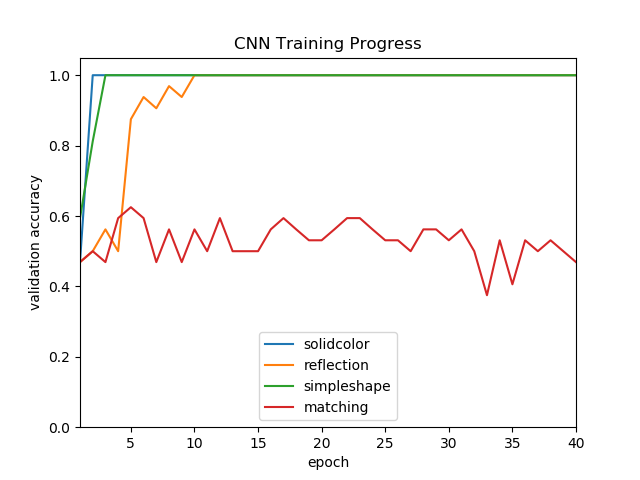
\includegraphics[width=\textwidth]{cnn-results.png}
\end{figure}

\subsection{GAN Results}




% TODO

\section{Conclusions}

There were some obvious shortcomings to this setup for comparing a CNN and a GAN.
The comparison is not apples-to-apples because the networks are designed in different ways as to require different types of inputs and present different types of outputs.
The CNN was given access to 1000 examples of class A and 1000 examples of class B, and so was classifying between two relatively-well-structured classes.
The GAN on the other hand was given access to just 1000 examples of class A, and the generator was expected to fill the role of providing examples of class B, and the discriminator just has to decide between class A and not class A which may not be as well-structured as class B depending on how the generator ends up looking.

Additionally, the CNN provided an exact measure of how well it classified images, but I was unable to program the GAN to provide an exact measure for how well it classified images of class A and B combined (so as to test both networks on the same total data set in the end).
This is certainly possible, but I was not knowledgeable about Tensorflow to successfuly implement this feature.
So, the results that I aquired are judged subjectively by how well the generator performed.

% TODO: what does this say about how well GANs solve the frame problem?

\end{document}
